% ICASSP 2027 submission draft. Every number in the results comes from
% results.tex, generated by scripts/product_paper_results.py from the run
% records in demo/nablafx_bench/ and the published appendix tables.
\documentclass{article}
\usepackage{spconf,amsmath,amssymb,graphicx,booktabs}
\usepackage[hidelinks]{hyperref}
\usepackage[T1]{fontenc}
\usepackage{times}

% Generated by scripts/product_paper_results.py; do not edit.
\newcommand{\pending}{\textbf{[pending]}}
\newcommand{\QuietLoudRatioRange}{2.6--4.2}
\newcommand{\PubSFourTFLesr}{0.108}
\newcommand{\PubSFourTFLparams}{70.2k}
\newcommand{\SSMparams}{11.3k}
\newcommand{\SSMparamsExact}{11{,}329}
\newcommand{\VoneSSMparamsExact}{12{,}353}
\newcommand{\SSMn}{3}
\newcommand{\SeedList}{42, 43 and 44}
\newcommand{\SSMesrMeanStd}{0.082\,{\scriptsize$\pm$\,0.046}}
\newcommand{\SSMmrstftMeanStd}{0.466\,{\scriptsize$\pm$\,0.072}}
\newcommand{\RerunSFourTFLesrMeanStd}{0.137\,{\scriptsize$\pm$\,0.020}}
\newcommand{\RerunSFourTFLn}{3}
\newcommand{\RerunSFourTFLlossGap}{8\,\%}
\newcommand{\ChangesSFourTFLesrMeanStd}{0.127\,{\scriptsize$\pm$\,0.035}}
\newcommand{\ChangesSFourTFLn}{3}
\newcommand{\SSMesrMin}{0.036}
\newcommand{\SSMesrMax}{0.128}
\newcommand{\ChangesSFourTFLesrMin}{0.089}
\newcommand{\ChangesSFourTFLesrMax}{0.157}
\newcommand{\ChangesSFourTFLmrstftMeanStd}{0.523\,{\scriptsize$\pm$\,0.032}}
\newcommand{\VoneSSMesr}{0.155\,{\scriptsize$\pm$\,0.115}}
\newcommand{\SSMpeakGiB}{17.2}
\newcommand{\SFourTFLpeakGiB}{16.3}
\newcommand{\GuardFlips}{10}
\newcommand{\GuardRuns}{6}
\newcommand{\GuardLastFlipEpoch}{11}
\newcommand{\InvertedStep}{5{,}100}
\newcommand{\InvertedEsr}{3.95}
\newcommand{\InvertedLone}{0.0286}
\newcommand{\InvertedNegatedEsr}{0.052}
\newcommand{\InvertedNegatedLone}{0.0035}
\newcommand{\TwiceMeanAbsTarget}{0.0299}
\newcommand{\PubOutliers}{TCN-2500-S-16, LSTM-32 and GCN-TF-2500-L-16}
\newcommand{\PubOutlierLoneRange}{0.0293--0.0295}
\newcommand{\RecurrenceDeviation}{3\times10^{-8}}
\newcommand{\ResultsTable}{\begin{table}[t]
\caption{Test results on the Big Muff under the NablAFx protocol, last checkpoint. Losses are unweighted. Our runs: mean $\pm$ standard deviation over $n$ seeds.}
\label{tab:results}
\smallskip
\centering\footnotesize\setlength{\tabcolsep}{3.5pt}
\begin{tabular}{@{}lrlll@{}}
\toprule
Model & Params & L1 ($10^{-3}$) & MR-STFT & ESR \\
\midrule
\multicolumn{5}{@{}l}{\emph{Published~\cite{comunita2025frontiers}}} \\
LSTM-96 & 38.1k & 3.3 & 0.523 & 0.120 \\
TCN-TF-2500-L-16 & 75.9k & 4.5 & 0.594 & 0.162 \\
GCN-TF-2500-S-16 & 154.1k & 4.3 & 0.594 & 0.137 \\
S4-S-16 & 2.4k & 4.8 & 0.643 & 0.237 \\
S4-L-16 & 19.0k & 4.2 & 0.596 & 0.192 \\
S4-TF-S-16 & 28.0k & 3.7 & 0.548 & 0.148 \\
S4-TF-L-16 & 70.2k & 3.1 & 0.505 & 0.108 \\
\midrule
\multicolumn{5}{@{}l}{\emph{Re-run, released training}} \\
S4-TF-L-16 ($n=3$) & 70.2k & 3.7\,{\scriptsize$\pm$\,0.6} & 0.544\,{\scriptsize$\pm$\,0.031} & 0.137\,{\scriptsize$\pm$\,0.020} \\
\midrule
\multicolumn{5}{@{}l}{\emph{Both training changes (Sec.~\ref{sec:setup})}} \\
S4-TF-L-16 ($n=3$) & 70.2k & 3.3\,{\scriptsize$\pm$\,0.5} & 0.523\,{\scriptsize$\pm$\,0.032} & 0.127\,{\scriptsize$\pm$\,0.035} \\
SSM-WaveNet ($n=3$) & 11.3k & 2.7\,{\scriptsize$\pm$\,0.6} & 0.466\,{\scriptsize$\pm$\,0.072} & 0.082\,{\scriptsize$\pm$\,0.046} \\
\midrule
\multicolumn{5}{@{}l}{\emph{Ablation: learned $b$, released training}} \\
SSM-WaveNet ($n=2$) & 12.4k & 3.6\,{\scriptsize$\pm$\,1.3} & 0.534\,{\scriptsize$\pm$\,0.099} & 0.155\,{\scriptsize$\pm$\,0.115} \\
\bottomrule
\end{tabular}
\end{table}}
\newcommand{\ChangesReduction}{7\,\%}
\newcommand{\ChangesPairedSeeds}{3}
\newcommand{\ChangesLowerSeeds}{2}
\newcommand{\SSMLowerThanVoneSeeds}{1}
\newcommand{\VoneLowerSeeds}{1}
\newcommand{\VonePairedSeeds}{2}
\newcommand{\SSMRatio}{1.5}
\newcommand{\ParamRatio}{6.2}
\newcommand{\SSMLowerSeeds}{3}
\newcommand{\PairedSeeds}{3}
\newcommand{\PubOffScale}{LSTM-32 (3.59), TCN-2500-S-16 (3.39), GCN-TF-2500-L-16 (3.61)}


\newcommand{\C}{\mathbb{C}}
\newcommand{\R}{\mathbb{R}}

\title{State-space WaveNets for compact black-box modelling of distortion effects}

% ORCiD 0009-0001-9266-786X (entered in the submission system).
\name{Antoine Lavault}
\address{LISTIC, Universit\'e Savoie Mont Blanc, France}

\begin{document}
\ninept
\maketitle

\begin{abstract}
Neural black-box models of guitar distortion either stack dilated causal
convolutions, as in the WaveNet-style models used in real-time plugins, or
chain state-space layers, which reach the best published accuracy on the
ToneTwist AFx benchmark when combined with temporal feature-wise modulation
(TFiLM). We propose SSM-WaveNet, a WaveNet whose dilated convolutions are
replaced by diagonal state-space layers, keeping its gated activations and skip
aggregation. Each layer is a bank of IIR filters that is stable by construction,
trained as a segment-long FFT convolution and run as a causal per-sample
recurrence. We train it inside the benchmark's public framework with two changes
to training, also applied to a re-run of the best published model: state-space
parameters are exempted from weight decay, as the framework's layers request,
and the output is negated whenever it anticorrelates with the validation target.
The second change is needed because the spectral term of the loss cannot see the
output's sign: one of our runs converged to an inverted output, and the test
errors of three published models show the same signature. On the Electro-Harmonix Big Muff,
a \SSMparams-parameter SSM-WaveNet reaches a test error-to-signal ratio of
\SSMesrMeanStd{} over \SSMn{} seeds, against \ChangesSFourTFLesrMeanStd{} for
the \PubSFourTFLparams-parameter S4-TFiLM model trained the same way and
\PubSFourTFLesr{} published.
\end{abstract}

\begin{keywords}
Virtual analog modelling, audio effects, state-space models, WaveNet, distortion
\end{keywords}

\section{Introduction}
\label{sec:intro}

Virtual analog modelling emulates analog audio circuits in software. Black-box
neural models learn the mapping from recordings of a device's input and output,
without knowledge of the circuit. Recurrent networks~\cite{wright2019realtime,
wright2020applsci} and WaveNet-style stacks of dilated causal
convolutions~\cite{vandenoord2016wavenet, damskagg2019icassp, damskagg2019smc}
run in real time; the latter is the architecture of the open-source Neural Amp
Modeler~\cite{atkinson2023nam}, widely used to capture guitar amplifiers and
pedals.

Comunit\`a et al.~\cite{comunita2025frontiers} compared LSTM, TCN, GCN and S4
models, with and without temporal feature-wise linear modulation
(TFiLM)~\cite{birnbaum2019tfilm, comunita2023icassp}, on 16 devices of the
ToneTwist AFx collection, using the open-source NablAFx
framework~\cite{comunita2025nablafx}. S4 models with TFiLM were the most
accurate overall; on the Big Muff fuzz pedal, the largest one reached a test
error-to-signal ratio (ESR) of \PubSFourTFLesr{} with \PubSFourTFLparams{}
parameters. Structured state-space models (SSMs)~\cite{gu2022s4, gupta2022dss,
gu2022s4d} have also been used for audio generation~\cite{goel2022sashimi}, to
model compressors~\cite{yin2024drc, simionato2025jaes}, and compared with
recurrent networks across several effect types~\cite{simionato2025ssm}. Closest
to our work, Esqueda and Murai~\cite{esqueda2025lru} interleave real linear
recurrent units with nonlinear stages to model distortion circuits.

The two families differ in more than their linear operator. WaveNet blocks gate
every layer with a tanh--sigmoid product and sum the layer outputs through skip
connections. The S4 models of~\cite{comunita2025frontiers} chain residual layers
with tanh activations and obtain long-range modulation from TFiLM, an LSTM
driven by max-pooled features. We ask whether the WaveNet topology, with its
dilated convolutions replaced by diagonal SSM layers, can do without TFiLM.
Unlike~\cite{esqueda2025lru}, our layers have complex, hence oscillatory, poles
and keep WaveNet's multiplicative gates and skip aggregation, and we compare
against the best published models under their own protocol. Our
contributions are:
(i)~SSM-WaveNet, a gated network whose layers are banks of stable IIR filters
and which runs as a causal per-sample recurrence (Sec.~\ref{sec:model});
(ii)~evidence that the L1 plus multi-resolution STFT loss of the benchmark
admits inverted solutions, reached by one of our runs and, judging from their
test errors, by three published models, and a polarity guard that prevents them
(Secs.~\ref{sec:setup} and~\ref{sec:discussion});
(iii)~a comparison inside NablAFx in which the best published model is re-run
both with the released training and with our training changes, with several
seeds per model (Sec.~\ref{sec:results}). Code, configurations and run records
are available at \url{https://github.com/ALavault/neural_amp}.

\section{SSM-WaveNet}
\label{sec:model}

\subsection{Diagonal state-space layer}

Let $u_c[t]$ be channel $c$ of a layer input. Each channel owns $N$ complex
states $s_{c,n}$ updated as
\begin{align}
s_{c,n}[t] &= p_{c,n}\, s_{c,n}[t-1] + b_{c,n}\, u_c[t], \label{eq:state}\\
v_c[t] &= 2\,\mathrm{Re}\Big(\textstyle\sum_{n=1}^{N} c_{c,n}\, s_{c,n}[t]\Big) + d_c\, u_c[t], \label{eq:out}
\end{align}
with learned $c_{c,n} \in \C$ and $d_c \in \R$. The poles are
$p_{c,n} = \exp(\lambda_{c,n}\Delta_c)$ with $\lambda_{c,n} = -e^{\alpha_{c,n}}
+ i\,\omega_{c,n}$ and $\Delta_c = e^{\delta_c}$, so that $|p_{c,n}| < 1$ for any
value of $\alpha$, $\omega$ and $\delta$: every layer is stable by construction.
The input weights follow from zero-order hold, $b_{c,n} = (p_{c,n} -
1)/\lambda_{c,n}$, which gives each mode the DC gain $-c_{c,n}/\lambda_{c,n}$
whatever the step $\Delta_c$. As in S4D-Lin~\cite{gu2022s4d} and the DSSM layer
of NablAFx, we initialise $\alpha_{c,n} = \log 0.5$, $\omega_{c,n} = \pi (n-1)$,
$\log\Delta_c$ uniformly in $[\log 10^{-3}, \log 10^{-1}]$ and $c_{c,n}$ from a
standard complex normal distribution; the layer is that DSSM layer except for
$d_c = 1$ at initialisation. Unrolling
(\ref{eq:state})--(\ref{eq:out}) gives $v_c = k_c * u_c + d_c u_c$ with the
impulse response
\begin{equation}
k_c[\tau] = 2\,\mathrm{Re}\textstyle\sum_{n=1}^{N} c_{c,n}\, b_{c,n}\, p_{c,n}^{\tau}, \qquad \tau \geq 0,
\label{eq:kernel}
\end{equation}
so each channel is a real IIR filter with $N$ conjugate pole pairs. During
training we evaluate $k_c$ over the whole segment and apply it with an FFT
convolution, so the memory is not truncated within a segment. At inference we
run (\ref{eq:state})--(\ref{eq:out}) sample by sample, at a cost of $O(N)$
operations per channel and without look-ahead. On 0.1\,s of test audio, the
recurrence reproduces the output of the FFT form of a trained network to within
$\RecurrenceDeviation$, computing in float64 except for a single-precision copy
of each layer input.

\subsection{Gated blocks}

An input $1\times1$ convolution maps the signal to $C$ channels $h_0$. Block $k$
applies an SSM layer to $h_{k-1}$, giving $v_k$, followed by a WaveNet gate and
two $1\times1$ projections:
\begin{align}
g_k &= \tanh(A_k v_k + a_k) \odot \sigma(B_k v_k + \beta_k), \label{eq:gate}\\
h_k &= h_{k-1} + R_k g_k + r_k, \qquad z_k = S_k g_k + \varsigma_k, \label{eq:res}
\end{align}
with $A_k, B_k, R_k, S_k \in \R^{C\times C}$. The skip outputs are summed and
mapped to the output sample by $\hat{y} = \tanh\big(W_2\,\phi(W_1\,
\phi(\sum_k z_k))\big)$, where $\phi$ is the ReLU and $W_1$, $W_2$ are $1\times1$
convolutions. The network therefore alternates stable linear filter banks with
memoryless gated nonlinearities and channel mixing, a learned and deep relative
of the block-oriented (Wiener--Hammerstein) models used for distortion
circuits, as are the LRU networks of~\cite{esqueda2025lru}. With $K$ blocks it
has $K(4C^2 + 4CN + 6C) + C^2 + 4C + 1$ parameters, and each output sample costs
$K(4C^2 + 3CN + 2C) + C^2 + 2C$ multiplications, counting a complex product as
one. We use $K=8$, $C=16$ and $N=4$: \SSMparamsExact{} parameters and 10{,}272
multiplications per sample. A first version learned $b$ instead of fixing it by
zero-order hold, with $b$ and $c$ initialised at a scale of 0.02
(\VoneSSMparamsExact{} parameters); we report it as an ablation.

The S4 blocks of NablAFx instead chain a linear map, a DSSM layer, a tanh, TFiLM
and a residual depthwise convolution. In that implementation, TFiLM computes the
modulation of each 128-sample block from the max-pooled features of the same
block, so streaming S4-TFiLM inference must buffer up to 127 samples
(2.6\,ms at 48\,kHz) or be retrained with a delayed modulation. SSM-WaveNet has
no pooling and no LSTM.

\section{Experimental setup}
\label{sec:setup}

\textbf{Data.} We use the Electro-Harmonix Big Muff recordings of Wright et
al.~\cite{wright2019realtime} (sustain 5, volume 10) distributed in ToneTwist
AFx~\cite{comunita2025tonetwist, wright2024tonetwistbigmuff} under CC~BY-NC~4.0: a 340\,s training and a
51\,s validation recording, and a 60\,s test recording with different musical
content, all mono at 44.1\,kHz. NablAFx resamples them to 48\,kHz, cuts training
and validation into 3\,s segments, pools them and draws a random 90/10 split
(118 training and 12 validation segments, since $1-0.9$ rounds below 0.1). The test recording is cut into
twelve 5\,s segments. Earlier results on these recordings~\cite{wright2019realtime}
follow a different protocol and are not comparable.

\textbf{Protocol.} All models are trained and tested with NablAFx (commit
\texttt{045db6e}) and the S4 training scheme of~\cite{comunita2025frontiers}:
AdamW with a learning rate of 0.01 and batch size 16, an L1 plus
multi-resolution STFT loss~\cite{steinmetz2020auraloss, yamamoto2020pwg},
gradient clipping at a value of 1, learning-rate halving after 20 epochs without
validation improvement, early stopping after 50, and at most 15k steps (the
released configuration file sets the clipping value to 10; we follow the
paper). As in the framework's released test script, test metrics are computed
on the last checkpoint, on each 5\,s segment with states reset, and averaged.
SSM-WaveNet uses the loss weights of the published S4-TF-L-16 (1 for L1, 0.1
for MR-STFT) and no hyperparameter search, whereas each published model is the
best of four loss weightings. Our changes to the framework's code read WAV files
with \texttt{soundfile} instead of a torchaudio loader removed in recent
versions, drop a logging flag removed from PyTorch, and log to CSV files
instead of Weights \& Biases. Runs use seeds \SeedList{} (42 is the framework
default); the seed changes the initialisation, the training/validation partition
and the batch order, while the test files are fixed.

\textbf{Training changes.} The DSSM layers of NablAFx, following the S4
reference code, mark $\alpha$, $\omega$ and $\delta$ as exempt from weight
decay, but the released training code puts all parameters in one AdamW group
with the default decay of 0.01. Decay pulls these log-parameters towards zero,
that is towards $\Delta_c = 1$ and $\mathrm{Re}\,\lambda_{c,n} = -1$, which
shortens the memory of every layer; we honour the exemption. Second, the
MR-STFT term is invariant to the sign of the output and, even at a weight of
0.1, stays 4 to 20 times larger than the L1 term on validation in our correctly
signed runs, so gradient descent can fit the spectrum with an inverted waveform.
SSM-WaveNet trained with the exemption alone did: after
\InvertedStep{} steps its test ESR was \InvertedEsr, and \InvertedNegatedEsr{}
with the output negated, and we stopped it. A polarity guard now computes, after
each validation epoch, the inner product of output and target over the
validation set; when it is negative, the guard negates the weight and bias of
the layer before the output tanh, which negates the output exactly, and their
Adam first moments. This uses one bit of validation information per epoch, less
than learning-rate scheduling and early stopping already use. We adopted the
exemption and zero-order hold after our first SSM-WaveNet run
(Table~\ref{tab:results}, ablation) had underperformed on the test set, choosing
them from its training and validation losses and its learned poles, and the
guard after the inversion, which validation had shown; the stopped run was
tested only to confirm it. Apart from the ablation and the
re-run labelled as released training, every run below uses both changes.

\textbf{Baselines.} We report the published Big Muff results of the best LSTM,
TCN and GCN models and of all four S4 variants~\cite{comunita2025frontiers}. We
re-run S4-TF-L-16, the best of them, with the same code as our model, once with
the released training and on each seed with our training changes.

\section{Results}
\label{sec:results}

\ResultsTable

\begin{figure}[t]
  \centering
  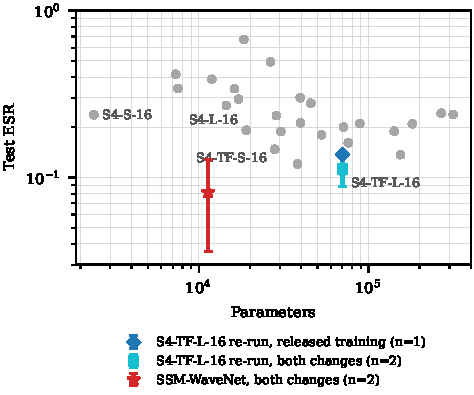
\includegraphics[width=\linewidth]{fig_pareto}
  \caption{Test ESR against parameter count on the Big Muff (log scales).
  Published black-box models of~\cite{comunita2025frontiers} in grey, S4
  variants labelled (off scale: \PubOffScale); re-runs and SSM-WaveNet show the
  mean and range over seeds.}
  \label{fig:pareto}
\end{figure}

Our re-run of S4-TF-L-16 with the released training reaches a test ESR of
\RerunSFourTFLesrMeanStd{} ($n=\RerunSFourTFLn$), against \PubSFourTFLesr{}
published, and an unweighted test loss \RerunSFourTFLlossGap{} above the
published one. The published value is the best of four loss weightings, whereas
the re-run trains the selected weighting once with the released framework. We
therefore compare SSM-WaveNet with re-runs, which share its code, data pipeline
and budget, and show the published values for context.

With both training changes, S4-TF-L-16 reaches a test ESR of
\ChangesSFourTFLesrMeanStd{} ($n=\ChangesSFourTFLn$), \ChangesReduction{} below
its re-run with the released training on the seeds trained both ways, but lower
on only \ChangesLowerSeeds{} of those \ChangesPairedSeeds{} seeds (published:
\PubSFourTFLesr): part of any difference between training recipes comes from the
seed, not from the recipe. SSM-WaveNet, trained the same way, reaches
\SSMesrMeanStd{} ($n=\SSMn$), \SSMRatio{} times lower than S4-TF-L-16 on average
and lower on \SSMLowerSeeds{} of \PairedSeeds{} paired seeds, with \ParamRatio{}
times fewer parameters, no TFiLM and no look-ahead; its MR-STFT loss is
\SSMmrstftMeanStd{}, against \ChangesSFourTFLmrstftMeanStd{} for S4-TF-L-16.
With a learned $b$ and the released training, the same network reaches only
\VoneSSMesr. Seeds matter more than one might expect on this benchmark: test ESR
spans \SSMesrMin{}--\SSMesrMax{} for SSM-WaveNet and
\ChangesSFourTFLesrMin{}--\ChangesSFourTFLesrMax{} for S4-TF-L-16, so a single
run tells little. Over the \GuardRuns{} guarded runs, the polarity guard fired
\GuardFlips{} times, never after epoch \GuardLastFlipEpoch.

\section{Discussion and limitations}
\label{sec:discussion}

\textbf{Inverted outputs.} An output $\hat{y} = -y$ has an L1 loss of
$2\,\mathrm{E}|y|$ whatever the model, \TwiceMeanAbsTarget{} on the test set; our
stopped run had \InvertedLone{} (\InvertedNegatedLone{} negated). The three
published neural models with a test ESR above 1, \PubOutliers, have L1 losses of
\PubOutlierLoneRange{} and MR-STFT losses within the range of the other models,
which is consistent with inverted but otherwise fitted outputs; we cannot
confirm it without their checkpoints. Any loss that compares magnitude spectra
alone has this symmetry, so training with one should check the sign of the
output on validation data.

\textbf{Limitations.} We evaluate a single device, while the published study
covers 16, with $n=\SSMn$ seeds per model, and the seed-to-seed spread is of the
same order as the difference between the two architectures. The training changes and zero-order hold were
chosen after a first SSM-WaveNet had underperformed on the test set; re-running
S4-TF-L-16 with the same changes controls for the changes, not for that choice.
Training evaluates each SSM kernel over the whole segment, which dominates
memory: a batch of sixteen 3\,s segments peaks at \SSMpeakGiB\,GiB on the GPU,
against \SFourTFLpeakGiB\,GiB for S4-TF-L-16. The per-sample cost given in
Sec.~\ref{sec:model} is analytical; we have not yet measured a compiled
real-time implementation.

\section{Conclusion}
\label{sec:conclusion}

On the Big Muff, SSM-WaveNet reaches a test ESR \SSMRatio{} times lower on
average than S4-TF-L-16, the most accurate published model, trained the same way
and lower on each of the \PairedSeeds{} seeds, with \ParamRatio{} times fewer
parameters, without TFiLM and without look-ahead. Whether this carries over to
the other devices of ToneTwist AFx and to a compiled real-time implementation
remains to be tested. The multi-resolution STFT loss used to
train and rank black-box effect models cannot see the sign of the output;
checking that sign on validation data costs nothing and should be part of such
benchmarks.

\section{Compliance with ethical standards}
This study uses publicly available recordings released under CC BY-NC 4.0 and
involves no human or animal subjects; no ethical approval was required.

\section{Acknowledgments}
% AI disclosure required by IEEE, confirmed by the author on 2026-09-15:
% https://open.ieee.org/author-guidelines-for-artificial-intelligence-ai-generated-text/
The author used Claude Opus 5 (Anthropic) to write the experiment and analysis
code, run the experiments and draft all sections of this paper. The author
reviewed and edited the text and checked the results against the run records.

\bibliographystyle{IEEEbib}
\bibliography{refs}

\end{document}
